\section[РСЛОС]{Регистр сдвига с линейной обратной связью}\label{section-lfsr}
\selectlanguage{russian}

Другой схемой построения псевдослучайных генераторов является использование регистров сдвига с линейной обратной связью, а также их вариациями. Для начала рассмотрим простой РСЛОС, изображённый на рисунке~\ref{fig:lfsr}.

\begin{figure}[thb]
	\centering
	\includegraphics[width=0.75\textwidth]{pic/lfsr}
	\caption{Регистр сдвига с линейной обратной связью}
	\label{fig:lfsr}
\end{figure}

Регистр сдвига состоит из $n$ однобитовых ячеек $b_1, b_2, \dots, b_n$, содержащих 0 или 1, и линейной обратной связи, определяемой коэффициентами $C_1 = 1$, $C_2, C_3, \dots, C_n \in \{0, 1\}$. Многочлен над полем GF(2) вида $C_1 x^n + C_2 x^{n-1} + \dots + C_n x + 1$ называется характеристическим многочленом РСЛОС.

Начальным состоянием генератора является набор значений в битовых ячейках. На каждой итерации генератор вычисляет сумму по модулю два (то есть выполняет операцию XOR) значений ячеек, для которых $C_i=1$:
\[\begin{array}{ll}
	b_{n+1} &= \sum\limits_{i} C_i b_i \mod 2, \\
	b_{n+1} &= b_1 \oplus C_2 b_2 \oplus C_3 b_3 \oplus \dots \oplus C_n b_n.
\end{array}\]

Далее регистр сдвигает значения на одну ячейку влево. Самая правая ячейчка $b_n$ принимает вычисленное значение $b_{n+1}$:
\[\begin{array}{ll}
	b_1 & := b_2, \\
	b_2 & := b_3, \\
	\dots \\
	b_n & := b_{n+1}. \\
\end{array}
\]

Выходом генератора является значение ячейки $b_1$ после сдвига.

\example
Пусть регистр сдвига с линейной обратной связью задан характеристическим многочленом $m\left(x\right)=x^{5} + x^{3} + 1$. Как показано на рисунке, регистр состоит из пяти ячееек. В линейной обратной связи будут участвовать ячейки 1 и 3 (то есть $C_1 = 1, C_3 = 1$, остальные $C_i = 0$).

\begin{center}
	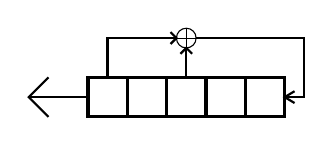
\begin{tikzpicture}[scale=0.05]
		\draw[black,very thick] (30,30) -- (30,40) -- (40,40) -- (40,30) -- (30,30) -- (30,40);
		\draw[black,thick] (35,40) -- (35,50) -- (35,50) -- (37.5,50);
		\draw[black,very thick] (40,30) -- (40,40) -- (50,40) -- (50,30) -- (40,30) -- (40,40);
		\draw[black,very thick] (50,30) -- (50,40) -- (60,40) -- (60,30) -- (50,30) -- (50,40);
		\draw[black,thick] (55,40) -- (55,47.5);
		\draw[black,thick] (53.5,46) -- (55,47.5) -- (56.5,46);
		\draw[black,thick] (37.5,50) -- (52.5,50);
		\draw[black,thick] (51,51.5) -- (52.5,50) -- (51,48.5);
		\draw (55,50) circle [radius=2.5];
		\draw[black] (52.5,50) -- (57.5,50);
		\draw[black] (55,47.5) -- (55,52.5);
		\draw[black,very thick] (60,30) -- (60,40) -- (70,40) -- (70,30) -- (60,30) -- (60,40);
		\draw[black,very thick] (70,30) -- (70,40) -- (80,40) -- (80,30) -- (70,30) -- (70,40);
		\draw[black,thick] (57.5,50) -- (85,50) -- (85,35) -- (80,35);
		\draw[black,thick] (82.5,36.5) -- (80,35) -- (82.5,33.5);
		\draw[black,thick] (30,35) -- (15,35);
		\draw[black,thick] (20,30) -- (15,35) -- (20,40);
	\end{tikzpicture}
\end{center}

Если начальное состояние регистра равно $\vec{s_0} = (0, 0, 0, 0, 1)$, то дальнейшие внутренние состояния регистра $s_i$ и выходы генератора $r_i$ равны:

\begin{enumerate}
	\item $b_{n+1} = b_1 \oplus b_3 = 0 \oplus 0 = 0$, $\vec{s_1} = (0, 0, 0, 1, 0)$, $r_1 = b_1 = 0$;
	\item $b_{n+1} = b_1 \oplus b_3 = 0 \oplus 0 = 0$, $\vec{s_2} = (0, 0, 1, 0, 0)$, $r_2 = b_1 = 0$;
	\item $b_{n+1} = b_1 \oplus b_3 = 0 \oplus 1 = 1$, $\vec{s_3} = (0, 1, 0, 0, 1)$, $r_3 = b_1 = 0$;
	\item $b_{n+1} = b_1 \oplus b_3 = 0 \oplus 0 = 0$, $\vec{s_4} = (1, 0, 0, 1, 0)$, $r_4 = b_1 = 1$;
	\item $b_{n+1} = b_1 \oplus b_3 = 1 \oplus 0 = 1$, $\vec{s_5} = (0, 0, 1, 0, 1)$, $r_5 = b_1 = 0$;
	\item $b_{n+1} = b_1 \oplus b_3 = 0 \oplus 1 = 0$, $\vec{s_6} = (0, 1, 0, 1, 0)$, $r_6 = b_1 = 0$;
	\item $b_{n+1} = b_1 \oplus b_3 = 0 \oplus 0 = 0$, $\vec{s_7} = (1, 0, 1, 0, 0)$, $r_7 = b_1 = 1$;
	\item $b_{n+1} = b_1 \oplus b_3 = 1 \oplus 1 = 0$, $\vec{s_8} = (0, 1, 0, 0, 0)$, $r_8 = b_1 = 0$;
	\item и так далее.
\end{enumerate}

\exampleend

Максимальный период последовательности РСЛОС равен $2^n - 1$. Максимум достигается в том и только том случае, когда характеристический многочлен РСЛОС примитивен. В этом случае РСЛОС называют регистром сдвига максимального периода, а генерируемые им последовательности -- М-последовательностями, или же последовательностями максимального периода.

Если известна структура РСЛОС (значения коэффициентов $C_2, \dots, C_n$), то внутреннее состояние генератора можно восстановить по $n$ предыдущим выходам. По $2n$ предыдущим выходам генератора можно восстановить и внутреннее состояние, и структуру генератора. Зная структуру и текущее внутреннее состояние генератора, можно восстановить его предыдущие и следующие выходные значения.
